% Created by tikzDevice version 0.10.1 on 2017-12-06 18:10:11
% !TEX encoding = UTF-8 Unicode
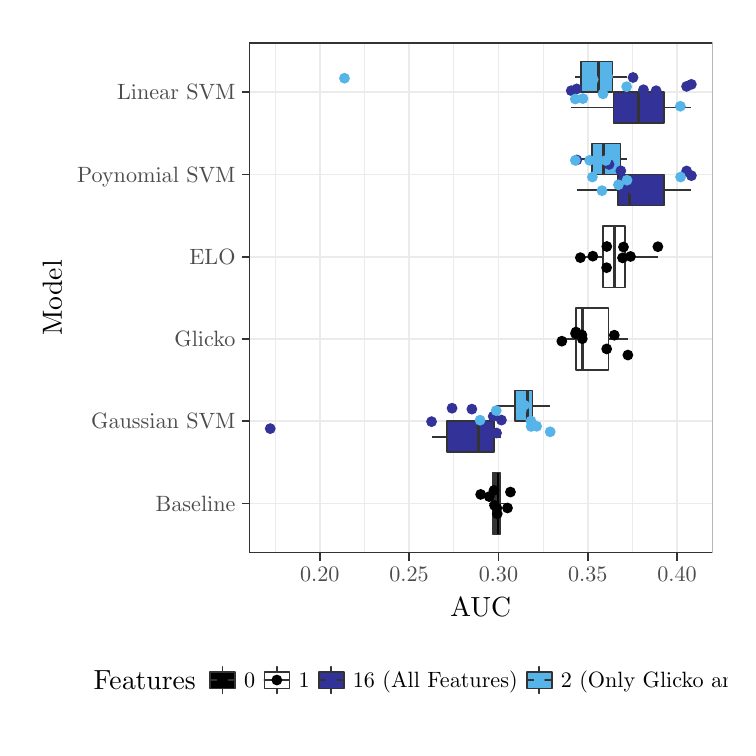
\begin{tikzpicture}[x=1pt,y=1pt]
\definecolor{fillColor}{RGB}{255,255,255}
\path[use as bounding box,fill=fillColor,fill opacity=0.00] (0,0) rectangle (252.94,252.94);
\begin{scope}
\path[clip] (  0.00,  0.00) rectangle (252.94,252.94);
\definecolor{drawColor}{RGB}{255,255,255}
\definecolor{fillColor}{RGB}{255,255,255}

\path[draw=drawColor,line width= 0.6pt,line join=round,line cap=round,fill=fillColor] (  0.00, -0.00) rectangle (252.94,252.94);
\end{scope}
\begin{scope}
\path[clip] ( 80.05, 63.15) rectangle (247.44,247.44);
\definecolor{fillColor}{RGB}{255,255,255}

\path[fill=fillColor] ( 80.05, 63.15) rectangle (247.44,247.45);
\definecolor{drawColor}{gray}{0.92}

\path[draw=drawColor,line width= 0.3pt,line join=round] ( 89.41, 63.15) --
	( 89.41,247.44);

\path[draw=drawColor,line width= 0.3pt,line join=round] (121.69, 63.15) --
	(121.69,247.44);

\path[draw=drawColor,line width= 0.3pt,line join=round] (153.97, 63.15) --
	(153.97,247.44);

\path[draw=drawColor,line width= 0.3pt,line join=round] (186.25, 63.15) --
	(186.25,247.44);

\path[draw=drawColor,line width= 0.3pt,line join=round] (218.53, 63.15) --
	(218.53,247.44);

\path[draw=drawColor,line width= 0.6pt,line join=round] ( 80.05, 80.99) --
	(247.44, 80.99);

\path[draw=drawColor,line width= 0.6pt,line join=round] ( 80.05,110.71) --
	(247.44,110.71);

\path[draw=drawColor,line width= 0.6pt,line join=round] ( 80.05,140.44) --
	(247.44,140.44);

\path[draw=drawColor,line width= 0.6pt,line join=round] ( 80.05,170.16) --
	(247.44,170.16);

\path[draw=drawColor,line width= 0.6pt,line join=round] ( 80.05,199.89) --
	(247.44,199.89);

\path[draw=drawColor,line width= 0.6pt,line join=round] ( 80.05,229.61) --
	(247.44,229.61);

\path[draw=drawColor,line width= 0.6pt,line join=round] (105.55, 63.15) --
	(105.55,247.44);

\path[draw=drawColor,line width= 0.6pt,line join=round] (137.83, 63.15) --
	(137.83,247.44);

\path[draw=drawColor,line width= 0.6pt,line join=round] (170.11, 63.15) --
	(170.11,247.44);

\path[draw=drawColor,line width= 0.6pt,line join=round] (202.39, 63.15) --
	(202.39,247.44);

\path[draw=drawColor,line width= 0.6pt,line join=round] (234.67, 63.15) --
	(234.67,247.44);
\definecolor{drawColor}{gray}{0.20}

\path[draw=drawColor,line width= 0.6pt,line join=round] (170.61, 80.99) -- (173.38, 80.99);

\path[draw=drawColor,line width= 0.6pt,line join=round] (168.07, 80.99) -- (166.80, 80.99);
\definecolor{fillColor}{RGB}{0,0,0}

\path[draw=drawColor,line width= 0.6pt,line join=round,line cap=round,fill=fillColor] (170.61, 69.84) --
	(168.07, 69.84) --
	(168.07, 92.14) --
	(170.61, 92.14) --
	(170.61, 69.84) --
	cycle;

\path[draw=drawColor,line width= 1.1pt,line join=round] (169.11, 69.84) -- (169.11, 92.14);

\path[draw=drawColor,line width= 0.6pt,line join=round] (168.51,105.14) -- (171.19,105.14);

\path[draw=drawColor,line width= 0.6pt,line join=round] (151.49,105.14) -- (145.93,105.14);
\definecolor{fillColor}{RGB}{50,50,153}

\path[draw=drawColor,line width= 0.6pt,line join=round,line cap=round,fill=fillColor] (168.51, 99.57) --
	(151.49, 99.57) --
	(151.49,110.71) --
	(168.51,110.71) --
	(168.51, 99.57) --
	cycle;

\path[draw=drawColor,line width= 1.1pt,line join=round] (163.05, 99.57) -- (163.05,110.71);

\path[draw=drawColor,line width= 0.6pt,line join=round] (182.41,116.29) -- (188.81,116.29);

\path[draw=drawColor,line width= 0.6pt,line join=round] (176.06,116.29) -- (169.30,116.29);
\definecolor{fillColor}{RGB}{86,180,233}

\path[draw=drawColor,line width= 0.6pt,line join=round,line cap=round,fill=fillColor] (182.41,110.71) --
	(176.06,110.71) --
	(176.06,121.86) --
	(182.41,121.86) --
	(182.41,110.71) --
	cycle;

\path[draw=drawColor,line width= 1.1pt,line join=round] (180.67,110.71) -- (180.67,121.86);

\path[draw=drawColor,line width= 0.6pt,line join=round] (209.90,140.44) -- (216.89,140.44);

\path[draw=drawColor,line width= 0.6pt,line join=round] (198.09,140.44) -- (193.02,140.44);
\definecolor{fillColor}{RGB}{255,255,255}

\path[draw=drawColor,line width= 0.6pt,line join=round,line cap=round,fill=fillColor] (209.90,129.29) --
	(198.09,129.29) --
	(198.09,151.58) --
	(209.90,151.58) --
	(209.90,129.29) --
	cycle;

\path[draw=drawColor,line width= 1.1pt,line join=round] (200.33,129.29) -- (200.33,151.58);

\path[draw=drawColor,line width= 0.6pt,line join=round] (215.94,170.16) -- (227.72,170.16);

\path[draw=drawColor,line width= 0.6pt,line join=round] (207.95,170.16) -- (199.72,170.16);

\path[draw=drawColor,line width= 0.6pt,line join=round,line cap=round,fill=fillColor] (215.94,159.02) --
	(207.95,159.02) --
	(207.95,181.31) --
	(215.94,181.31) --
	(215.94,159.02) --
	cycle;

\path[draw=drawColor,line width= 1.1pt,line join=round] (212.10,159.02) -- (212.10,181.31);

\path[draw=drawColor,line width= 0.6pt,line join=round] (229.84,194.31) -- (239.83,194.31);

\path[draw=drawColor,line width= 0.6pt,line join=round] (213.26,194.31) -- (198.43,194.31);
\definecolor{fillColor}{RGB}{50,50,153}

\path[draw=drawColor,line width= 0.6pt,line join=round,line cap=round,fill=fillColor] (229.84,188.74) --
	(213.26,188.74) --
	(213.26,199.89) --
	(229.84,199.89) --
	(229.84,188.74) --
	cycle;

\path[draw=drawColor,line width= 1.1pt,line join=round] (217.46,188.74) -- (217.46,199.89);

\path[draw=drawColor,line width= 0.6pt,line join=round] (214.24,205.46) -- (216.59,205.46);

\path[draw=drawColor,line width= 0.6pt,line join=round] (203.82,205.46) -- (197.88,205.46);
\definecolor{fillColor}{RGB}{86,180,233}

\path[draw=drawColor,line width= 0.6pt,line join=round,line cap=round,fill=fillColor] (214.24,199.89) --
	(203.82,199.89) --
	(203.82,211.03) --
	(214.24,211.03) --
	(214.24,199.89) --
	cycle;

\path[draw=drawColor,line width= 1.1pt,line join=round] (208.21,199.89) -- (208.21,211.03);

\path[draw=drawColor,line width= 0.6pt,line join=round] (229.84,224.04) -- (239.83,224.04);

\path[draw=drawColor,line width= 0.6pt,line join=round] (211.73,224.04) -- (196.41,224.04);
\definecolor{fillColor}{RGB}{50,50,153}

\path[draw=drawColor,line width= 0.6pt,line join=round,line cap=round,fill=fillColor] (229.84,218.46) --
	(211.73,218.46) --
	(211.73,229.61) --
	(229.84,229.61) --
	(229.84,218.46) --
	cycle;

\path[draw=drawColor,line width= 1.1pt,line join=round] (220.64,218.46) -- (220.64,229.61);

\path[draw=drawColor,line width= 0.6pt,line join=round] (211.29,235.18) -- (216.44,235.18);

\path[draw=drawColor,line width= 0.6pt,line join=round] (199.94,235.18) -- (197.88,235.18);
\definecolor{fillColor}{RGB}{86,180,233}

\path[draw=drawColor,line width= 0.6pt,line join=round,line cap=round,fill=fillColor] (211.29,229.61) --
	(199.94,229.61) --
	(199.94,240.76) --
	(211.29,240.76) --
	(211.29,229.61) --
	cycle;

\path[draw=drawColor,line width= 1.1pt,line join=round] (206.13,229.61) -- (206.13,240.76);
\definecolor{fillColor}{RGB}{0,0,0}

\path[fill=fillColor] (163.68, 84.28) circle (  1.96);

\path[fill=fillColor] (169.54, 79.32) circle (  1.96);

\path[fill=fillColor] (166.79, 83.50) circle (  1.96);

\path[fill=fillColor] (169.68, 77.28) circle (  1.96);

\path[fill=fillColor] (168.50, 85.74) circle (  1.96);

\path[fill=fillColor] (174.45, 85.14) circle (  1.96);

\path[fill=fillColor] (173.39, 79.38) circle (  1.96);

\path[fill=fillColor] (168.69, 80.32) circle (  1.96);

\path[fill=fillColor] (204.22,170.37) circle (  1.96);

\path[fill=fillColor] (215.29,173.67) circle (  1.96);

\path[fill=fillColor] (199.72,169.84) circle (  1.96);

\path[fill=fillColor] (209.27,173.87) circle (  1.96);

\path[fill=fillColor] (217.84,170.26) circle (  1.96);

\path[fill=fillColor] (214.94,169.76) circle (  1.96);

\path[fill=fillColor] (209.20,166.21) circle (  1.96);

\path[fill=fillColor] (227.73,173.79) circle (  1.96);
\definecolor{fillColor}{RGB}{50,50,153}

\path[fill=fillColor] (168.22,112.49) circle (  1.96);

\path[fill=fillColor] (169.43,106.48) circle (  1.96);

\path[fill=fillColor] (165.59,108.98) circle (  1.96);

\path[fill=fillColor] (145.94,110.58) circle (  1.96);

\path[fill=fillColor] (153.35,115.43) circle (  1.96);

\path[fill=fillColor] (171.19,111.14) circle (  1.96);

\path[fill=fillColor] (160.51,115.10) circle (  1.96);

\path[fill=fillColor] ( 87.65,108.06) circle (  1.96);
\definecolor{fillColor}{RGB}{86,180,233}

\path[fill=fillColor] (183.92,108.90) circle (  1.96);

\path[fill=fillColor] (188.81,106.90) circle (  1.96);

\path[fill=fillColor] (178.32,114.41) circle (  1.96);

\path[fill=fillColor] (179.49,116.54) circle (  1.96);

\path[fill=fillColor] (163.47,111.09) circle (  1.96);

\path[fill=fillColor] (181.92,108.85) circle (  1.96);

\path[fill=fillColor] (181.85,110.79) circle (  1.96);

\path[fill=fillColor] (169.30,114.56) circle (  1.96);
\definecolor{fillColor}{RGB}{0,0,0}

\path[fill=fillColor] (198.13,142.95) circle (  1.96);

\path[fill=fillColor] (200.26,141.92) circle (  1.96);

\path[fill=fillColor] (193.01,139.65) circle (  1.96);

\path[fill=fillColor] (216.88,134.64) circle (  1.96);

\path[fill=fillColor] (211.98,141.82) circle (  1.96);

\path[fill=fillColor] (197.98,142.36) circle (  1.96);

\path[fill=fillColor] (209.22,136.85) circle (  1.96);

\path[fill=fillColor] (200.41,140.53) circle (  1.96);
\definecolor{fillColor}{RGB}{50,50,153}

\path[fill=fillColor] (227.09,230.15) circle (  1.96);

\path[fill=fillColor] (196.42,230.17) circle (  1.96);

\path[fill=fillColor] (216.17,227.72) circle (  1.96);

\path[fill=fillColor] (198.42,230.81) circle (  1.96);

\path[fill=fillColor] (218.75,234.94) circle (  1.96);

\path[fill=fillColor] (222.51,230.50) circle (  1.96);

\path[fill=fillColor] (238.09,231.71) circle (  1.96);

\path[fill=fillColor] (239.82,232.45) circle (  1.96);
\definecolor{fillColor}{RGB}{86,180,233}

\path[fill=fillColor] (204.36,234.21) circle (  1.96);

\path[fill=fillColor] (216.44,231.61) circle (  1.96);

\path[fill=fillColor] (207.90,229.02) circle (  1.96);

\path[fill=fillColor] (114.47,234.67) circle (  1.96);

\path[fill=fillColor] (197.87,227.16) circle (  1.96);

\path[fill=fillColor] (200.63,227.30) circle (  1.96);

\path[fill=fillColor] (209.57,235.34) circle (  1.96);

\path[fill=fillColor] (235.85,224.54) circle (  1.96);
\definecolor{fillColor}{RGB}{50,50,153}

\path[fill=fillColor] (218.77,194.38) circle (  1.96);

\path[fill=fillColor] (198.43,205.14) circle (  1.96);

\path[fill=fillColor] (227.08,195.28) circle (  1.96);

\path[fill=fillColor] (216.17,197.03) circle (  1.96);

\path[fill=fillColor] (214.33,201.21) circle (  1.96);

\path[fill=fillColor] (239.84,199.46) circle (  1.96);

\path[fill=fillColor] (210.08,203.52) circle (  1.96);

\path[fill=fillColor] (238.10,201.16) circle (  1.96);
\definecolor{fillColor}{RGB}{86,180,233}

\path[fill=fillColor] (207.52,194.04) circle (  1.96);

\path[fill=fillColor] (204.06,198.97) circle (  1.96);

\path[fill=fillColor] (216.58,197.83) circle (  1.96);

\path[fill=fillColor] (235.93,198.97) circle (  1.96);

\path[fill=fillColor] (208.91,204.96) circle (  1.96);

\path[fill=fillColor] (197.88,204.99) circle (  1.96);

\path[fill=fillColor] (213.46,196.17) circle (  1.96);

\path[fill=fillColor] (203.06,205.00) circle (  1.96);

\path[draw=drawColor,line width= 0.6pt,line join=round,line cap=round] ( 80.05, 63.15) rectangle (247.44,247.45);
\end{scope}
\begin{scope}
\path[clip] (  0.00,  0.00) rectangle (252.94,252.94);
\definecolor{drawColor}{gray}{0.30}

\node[text=drawColor,anchor=base east,inner sep=0pt, outer sep=0pt, scale=  0.80] at ( 75.10, 78.23) {Baseline};

\node[text=drawColor,anchor=base east,inner sep=0pt, outer sep=0pt, scale=  0.80] at ( 75.10,107.96) {Gaussian SVM};

\node[text=drawColor,anchor=base east,inner sep=0pt, outer sep=0pt, scale=  0.80] at ( 75.10,137.68) {Glicko};

\node[text=drawColor,anchor=base east,inner sep=0pt, outer sep=0pt, scale=  0.80] at ( 75.10,167.41) {ELO};

\node[text=drawColor,anchor=base east,inner sep=0pt, outer sep=0pt, scale=  0.80] at ( 75.10,197.13) {Poynomial SVM};

\node[text=drawColor,anchor=base east,inner sep=0pt, outer sep=0pt, scale=  0.80] at ( 75.10,226.86) {Linear SVM};
\end{scope}
\begin{scope}
\path[clip] (  0.00,  0.00) rectangle (252.94,252.94);
\definecolor{drawColor}{gray}{0.20}

\path[draw=drawColor,line width= 0.6pt,line join=round] ( 77.30, 80.99) --
	( 80.05, 80.99);

\path[draw=drawColor,line width= 0.6pt,line join=round] ( 77.30,110.71) --
	( 80.05,110.71);

\path[draw=drawColor,line width= 0.6pt,line join=round] ( 77.30,140.44) --
	( 80.05,140.44);

\path[draw=drawColor,line width= 0.6pt,line join=round] ( 77.30,170.16) --
	( 80.05,170.16);

\path[draw=drawColor,line width= 0.6pt,line join=round] ( 77.30,199.89) --
	( 80.05,199.89);

\path[draw=drawColor,line width= 0.6pt,line join=round] ( 77.30,229.61) --
	( 80.05,229.61);
\end{scope}
\begin{scope}
\path[clip] (  0.00,  0.00) rectangle (252.94,252.94);
\definecolor{drawColor}{gray}{0.20}

\path[draw=drawColor,line width= 0.6pt,line join=round] (105.55, 60.40) --
	(105.55, 63.15);

\path[draw=drawColor,line width= 0.6pt,line join=round] (137.83, 60.40) --
	(137.83, 63.15);

\path[draw=drawColor,line width= 0.6pt,line join=round] (170.11, 60.40) --
	(170.11, 63.15);

\path[draw=drawColor,line width= 0.6pt,line join=round] (202.39, 60.40) --
	(202.39, 63.15);

\path[draw=drawColor,line width= 0.6pt,line join=round] (234.67, 60.40) --
	(234.67, 63.15);
\end{scope}
\begin{scope}
\path[clip] (  0.00,  0.00) rectangle (252.94,252.94);
\definecolor{drawColor}{gray}{0.30}

\node[text=drawColor,anchor=base,inner sep=0pt, outer sep=0pt, scale=  0.80] at (105.55, 52.69) {0.20};

\node[text=drawColor,anchor=base,inner sep=0pt, outer sep=0pt, scale=  0.80] at (137.83, 52.69) {0.25};

\node[text=drawColor,anchor=base,inner sep=0pt, outer sep=0pt, scale=  0.80] at (170.11, 52.69) {0.30};

\node[text=drawColor,anchor=base,inner sep=0pt, outer sep=0pt, scale=  0.80] at (202.39, 52.69) {0.35};

\node[text=drawColor,anchor=base,inner sep=0pt, outer sep=0pt, scale=  0.80] at (234.67, 52.69) {0.40};
\end{scope}
\begin{scope}
\path[clip] (  0.00,  0.00) rectangle (252.94,252.94);
\definecolor{drawColor}{RGB}{0,0,0}

\node[text=drawColor,anchor=base,inner sep=0pt, outer sep=0pt, scale=  1.00] at (163.75, 40.31) {AUC};
\end{scope}
\begin{scope}
\path[clip] (  0.00,  0.00) rectangle (252.94,252.94);
\definecolor{drawColor}{RGB}{0,0,0}

\node[text=drawColor,rotate= 90.00,anchor=base,inner sep=0pt, outer sep=0pt, scale=  1.00] at ( 12.39,155.30) {Model};
\end{scope}
\begin{scope}
\path[clip] (  0.00,  0.00) rectangle (252.94,252.94);
\definecolor{fillColor}{RGB}{255,255,255}

\path[fill=fillColor] ( 18.18,  5.50) rectangle (309.31, 28.93);
\end{scope}
\begin{scope}
\path[clip] (  0.00,  0.00) rectangle (252.94,252.94);
\definecolor{drawColor}{RGB}{0,0,0}

\node[text=drawColor,anchor=base west,inner sep=0pt, outer sep=0pt, scale=  1.00] at ( 23.87, 13.77) {Features};
\end{scope}
\begin{scope}
\path[clip] (  0.00,  0.00) rectangle (252.94,252.94);
\definecolor{fillColor}{RGB}{255,255,255}

\path[fill=fillColor] ( 64.36, 11.19) rectangle ( 76.41, 23.24);
\end{scope}
\begin{scope}
\path[clip] (  0.00,  0.00) rectangle (252.94,252.94);
\definecolor{drawColor}{gray}{0.20}

\path[draw=drawColor,line width= 0.6pt,line join=round,line cap=round] ( 70.38, 12.40) --
	( 70.38, 14.20);

\path[draw=drawColor,line width= 0.6pt,line join=round,line cap=round] ( 70.38, 20.22) --
	( 70.38, 22.03);
\definecolor{fillColor}{RGB}{0,0,0}

\path[draw=drawColor,line width= 0.6pt,line join=round,line cap=round,fill=fillColor] ( 65.87, 14.20) rectangle ( 74.90, 20.22);

\path[draw=drawColor,line width= 0.6pt,line join=round,line cap=round] ( 65.87, 17.21) --
	( 74.90, 17.21);
\end{scope}
\begin{scope}
\path[clip] (  0.00,  0.00) rectangle (252.94,252.94);
\definecolor{fillColor}{RGB}{0,0,0}

\path[fill=fillColor] ( 70.38, 17.21) circle (  1.96);
\end{scope}
\begin{scope}
\path[clip] (  0.00,  0.00) rectangle (252.94,252.94);
\definecolor{fillColor}{RGB}{255,255,255}

\path[fill=fillColor] ( 84.02, 11.19) rectangle ( 96.06, 23.24);
\end{scope}
\begin{scope}
\path[clip] (  0.00,  0.00) rectangle (252.94,252.94);
\definecolor{drawColor}{gray}{0.20}

\path[draw=drawColor,line width= 0.6pt,line join=round,line cap=round] ( 90.04, 12.40) --
	( 90.04, 14.20);

\path[draw=drawColor,line width= 0.6pt,line join=round,line cap=round] ( 90.04, 20.22) --
	( 90.04, 22.03);
\definecolor{fillColor}{RGB}{255,255,255}

\path[draw=drawColor,line width= 0.6pt,line join=round,line cap=round,fill=fillColor] ( 85.52, 14.20) rectangle ( 94.56, 20.22);

\path[draw=drawColor,line width= 0.6pt,line join=round,line cap=round] ( 85.52, 17.21) --
	( 94.56, 17.21);
\end{scope}
\begin{scope}
\path[clip] (  0.00,  0.00) rectangle (252.94,252.94);
\definecolor{fillColor}{RGB}{0,0,0}

\path[fill=fillColor] ( 90.04, 17.21) circle (  1.96);
\end{scope}
\begin{scope}
\path[clip] (  0.00,  0.00) rectangle (252.94,252.94);
\definecolor{fillColor}{RGB}{255,255,255}

\path[fill=fillColor] (103.68, 11.19) rectangle (115.72, 23.24);
\end{scope}
\begin{scope}
\path[clip] (  0.00,  0.00) rectangle (252.94,252.94);
\definecolor{drawColor}{gray}{0.20}

\path[draw=drawColor,line width= 0.6pt,line join=round,line cap=round] (109.70, 12.40) --
	(109.70, 14.20);

\path[draw=drawColor,line width= 0.6pt,line join=round,line cap=round] (109.70, 20.22) --
	(109.70, 22.03);
\definecolor{fillColor}{RGB}{50,50,153}

\path[draw=drawColor,line width= 0.6pt,line join=round,line cap=round,fill=fillColor] (105.18, 14.20) rectangle (114.22, 20.22);

\path[draw=drawColor,line width= 0.6pt,line join=round,line cap=round] (105.18, 17.21) --
	(114.22, 17.21);
\end{scope}
\begin{scope}
\path[clip] (  0.00,  0.00) rectangle (252.94,252.94);
\definecolor{fillColor}{RGB}{50,50,153}

\path[fill=fillColor] (109.70, 17.21) circle (  1.96);
\end{scope}
\begin{scope}
\path[clip] (  0.00,  0.00) rectangle (252.94,252.94);
\definecolor{fillColor}{RGB}{255,255,255}

\path[fill=fillColor] (178.83, 11.19) rectangle (190.88, 23.24);
\end{scope}
\begin{scope}
\path[clip] (  0.00,  0.00) rectangle (252.94,252.94);
\definecolor{drawColor}{gray}{0.20}

\path[draw=drawColor,line width= 0.6pt,line join=round,line cap=round] (184.85, 12.40) --
	(184.85, 14.20);

\path[draw=drawColor,line width= 0.6pt,line join=round,line cap=round] (184.85, 20.22) --
	(184.85, 22.03);
\definecolor{fillColor}{RGB}{86,180,233}

\path[draw=drawColor,line width= 0.6pt,line join=round,line cap=round,fill=fillColor] (180.34, 14.20) rectangle (189.37, 20.22);

\path[draw=drawColor,line width= 0.6pt,line join=round,line cap=round] (180.34, 17.21) --
	(189.37, 17.21);
\end{scope}
\begin{scope}
\path[clip] (  0.00,  0.00) rectangle (252.94,252.94);
\definecolor{fillColor}{RGB}{86,180,233}

\path[fill=fillColor] (184.85, 17.21) circle (  1.96);
\end{scope}
\begin{scope}
\path[clip] (  0.00,  0.00) rectangle (252.94,252.94);
\definecolor{drawColor}{RGB}{0,0,0}

\node[text=drawColor,anchor=base west,inner sep=0pt, outer sep=0pt, scale=  0.80] at ( 78.21, 14.46) {0};
\end{scope}
\begin{scope}
\path[clip] (  0.00,  0.00) rectangle (252.94,252.94);
\definecolor{drawColor}{RGB}{0,0,0}

\node[text=drawColor,anchor=base west,inner sep=0pt, outer sep=0pt, scale=  0.80] at ( 97.87, 14.46) {1};
\end{scope}
\begin{scope}
\path[clip] (  0.00,  0.00) rectangle (252.94,252.94);
\definecolor{drawColor}{RGB}{0,0,0}

\node[text=drawColor,anchor=base west,inner sep=0pt, outer sep=0pt, scale=  0.80] at (117.53, 14.46) {16 (All Features)};
\end{scope}
\begin{scope}
\path[clip] (  0.00,  0.00) rectangle (252.94,252.94);
\definecolor{drawColor}{RGB}{0,0,0}

\node[text=drawColor,anchor=base west,inner sep=0pt, outer sep=0pt, scale=  0.80] at (192.68, 14.46) {2 (Only Glicko and ELO Score)};
\end{scope}
\end{tikzpicture}
